% Copyright (c)  2005-2010 EDF-EADS-PHIMECA.
% Permission is granted to copy, distribute and/or modify this document
% under the terms of the GNU Free Documentation License, Version 1.2
% or any later version published by the Free Software Foundation;
% with no Invariant Sections, no Front-Cover Texts, and no Back-Cover
% Texts.  A copy of the license is included in the section entitled "GNU
% Free Documentation License".
% This chapter deals with the software architecture of the \OT\ platform. It follows the functional architecture which offered a global, rather general and coarse-grained view of the constituent bricks. Here, we will address technical considerations regarding development, feasability, performance, upgradability, and so on, by declining the concepts as programming classes and objects. At this level, the interaction with the technical architecture is strong since the technical choices have a direct influence on the design model.

Before describing in detail the design of each class (package after package), this chapter introduces a few design models that are widely used within the \OT\ platform.

\section{Notation and glossary}

The presentation of the design model relies on a graphical UML notation (see [UML]) that needs to be introduced for the readers who may not yet be familiar with this type of representation. This notation largely draws upon the one used for the analysis, especially as far as associations are concerned, but it needs to be supplemented to take into account the new elements (which will be described afterwards). Please refer to section \ref{notations} for the notations that were already introduced.

\subsection{Class}

The class is the natural entity that materializes the analysis concept. It is a type that defines the behavior of any object belonging to the class. It is represented by a rectangle horizontally divided into three parts: in the top part is the name of the class; the middle section gives the list of attributes; the bottom part contains the list of methods. The attribute and method sections are optional (see Figure \ref{fig:class}).

\begin{figure}[htb]
  \begin{center}
    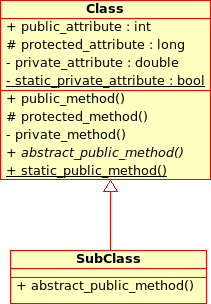
\includegraphics[scale=0.5]{Figures/modeling_notions/class.png}
    \caption{Representing classes.}\label{fig:class}
  \end{center}
\end{figure}

\subsection{Object}

An object is an instance of a class. It is graphically represented by a rectangle containing the name of the object and its class, separated by a colon (:) and underlined. When the name of the object is not significant, it can be omitted; the class can never be.

\subsection{Attribute}

The attribute is an internal element of the object or of the class that describes (partially or entirely) the state of the object. It is defined by a name, a type, a visibility and a scope.

\subsection{Method}

The method is an operation that affects an object or a class. It is the natural place to define how an object can be processed. The method is defined by a signature (see \cite{C++}), a visibility and a scope.

\subsection{Visibility}

Visibility defines the possibility of accessing an attribute or a method of a given class. There are three possible values:

\begin{itemize}
\item \emph{Public}: the attribute or method can be accessed by any object from any class.
\item \emph{Protected}: the attribute or method can be accessed by any object from a class deriving from the aforementioned class, but not by any other object .
\item \emph{Private}: the attribute or method can only be accessed by objects from the aforementioned class.
\end{itemize}


This (very simple) definition of visibility is the one given by the C++ language (see \cite{C++}), which is the language chosen for the platform's implementation. Other languages may have different definitions of visibility.

Visibility is graphically represented by a plus sign (+) for public, a hash sign (\#) for protected and a minus sign (-) for private.

\subsection{Scope}

An attribute or method belongs by default to the object instantiated from the class where it is defined. For example, the lifespan of a standard attribute is the same as the lifespan of the object carrying it. This behavior can be modified by declaring the object as static: its lifespan then become the same as the application's, and it can only be accessed through the class (and not through the object).

In the same way, a method that was declared static can no longer process objects instantiated from its class; it can only process the class itself and its static attributes.

The static scope of an attribute or a method is graphically represented by underlining the said attribute or method.

\subsection{Abstract class and method}

A class or a method can be defined as abstract. For a class, it means that it cannot (and should not) be instantiated and that there are no available objects belonging to this class. This class must be derived into a sub-class in order to be usable.

An abstract method is a method whose signature is declared but for which no definition has been given. A class with an abstract method is de facto abstract, since it cannot be instantiated due to the undefined method. In order to be able to derive the abstract class into a concrete sub-class, it is necessary to define the abstract method in the sub-class; if the abstract method is not defined, the abstract trait is propagated to the sub-class.

Graphically speaking, an abstract class or method is represented by a name or signature written in italic font.

\subsection{Method call}

The UML notation defines a representation of interactions between objects defined as class instances. This representation allows to visualize the links between these objects and the communication that they establish. It is shown in a collaboration diagram in which objects are represented as instances (and no longer as classes), and the links between objects support the name of a method issued from the calling object to the called object. Figure \ref{fig:collaboration} shows an example of such a diagram.

\begin{figure}[htb]
  \begin{center}
    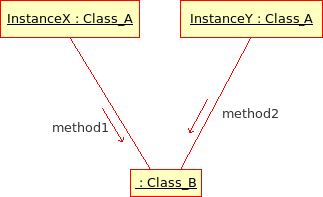
\includegraphics[scale=0.5]{Figures/modeling_notions/collaboration.png}
    \caption{Collaboration diagram.}\label{fig:collaboration}
  \end{center}
\end{figure}

\section{Design patterns}

\subsection{Introduction}

Software design shows the recurrence of some patterns, whether within the same piece of software or in several applications (which can differ in many ways). These patterns have been catalogued (\cite{GoF} can be referred to with great benefit on this subject), described and implemented in numerous situations that prove their universality and their ability to solve recurring problems that the software architect is faced with.

The following sections give an overview intended as much for the reader's understanding of the document as to establish a common vocabulary for software architect. The latter ones will find here standard design diagrams applied to the specific case of \OT, which can help them better apprehend the tool's specificities and the design and implementation choices that were made.

\label{singleton}\subsection{Singleton pattern}

The Singleton is a pattern used to ensure that at any given time, there is only one instance of a class (A); it provides an access point for this unique instance.

This is implemented by creating a class (Singleton) with a static private attribute (uniqueInstance) initialized with an instance of class A and whose reference (or pointer) is returned by a static method (instance). Figure \ref{fig:singleton} illustrates the Singleton pattern.

\begin{figure}[htb]
  \begin{center}
    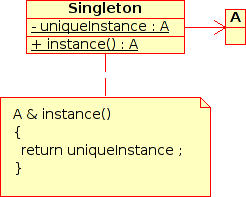
\includegraphics[scale=0.5]{Figures/modeling_notions/singleton.png}
    \caption{Singleton structure.}\label{fig:singleton}
  \end{center}
\end{figure}

It is a very common pattern that allows to find and share an object (which must remain unique) in different portions of code. Examples of such objects include shared hardware resources (standard output, error, log, etc.), but also internal functions that cannot or must not be duplicated (e.g. a random number generator).

\label{factory}\subsection{Factory pattern}

This pattern allows to define a unique interface for the creation of objects belonging to a class hierarchy withouth knowing in advance their exact type. Figure \ref{fig:factory} illustrates this pattern. The creation of the concrete object (ClassA or ClassB) is delegated to a sub-class (ClassAFactory or ClassBFactory) which chooses the type of object to be created and the strategy to be used to create it.

\begin{figure}[htb]
  \begin{center}
    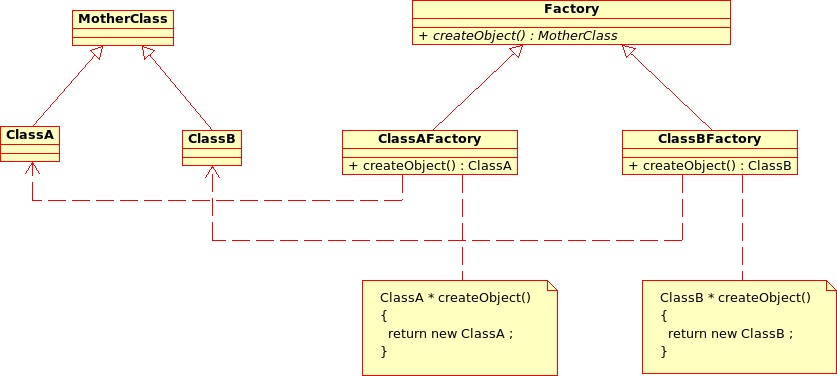
\includegraphics[scale=0.5]{Figures/modeling_notions/factory.png}
    \caption{Factory structure.}\label{fig:factory}
  \end{center}
\end{figure}

This pattern is often used to dynamically create objects belonging to related types (e.g. to instantiate objects within a GUI according to the user's behavior). It can also be used to back up and read again a document written in a file by automatically re-instantiating objects. It is a pattern that makes code maintenance easier by clearly separating the objects and their instantiation in distinct and parallel class hierarchies.

\label{strategy}\subsection{Strategy pattern}

The Strategy pattern defines a family of algorithm and makes them interchangeable as far as the client is concerned. Access to these algorithms is provided by a unique interface which encapsulates the algorithms' implementation. Therefore, the implementation can change without the client being aware of it.

\begin{figure}[htb]
  \begin{center}
    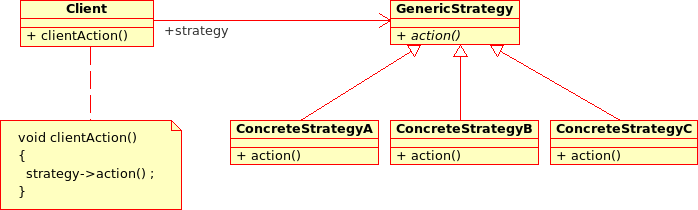
\includegraphics[scale=0.5]{Figures/modeling_notions/strategy.png}
    \caption{Strategy structure.}\label{fig:strategy}
  \end{center}
\end{figure}

This pattern is very useful to provide a client with different implementations of an algorithm which are equivalent from a functional point of view. It can be noted that the Factory pattern described earlier makes use of the Strategy pattern.

\label{composite}\subsection{Composite pattern}

The Composite pattern is used to organize objects into a tree structure that represents the hierarchies between component and composite objects. It hides the complex structure of the object from the client handling the object.

\begin{figure}[htb]
  \begin{center}
    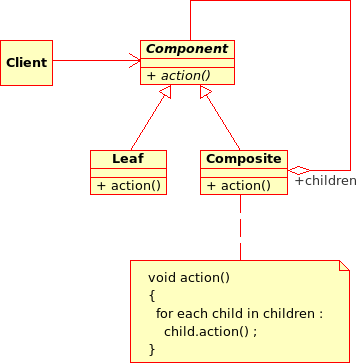
\includegraphics[scale=0.5]{Figures/modeling_notions/composite.png}
    \caption{Composite structure.}\label{fig:composite}
  \end{center}
\end{figure}

Figure \ref{fig:composite_tree} shows an example of tree modeled by the Composite. The Composite objects make up the tree nodes whereas the leaves can be any concrete object deriving from Component.

\begin{figure}[htb]
  \begin{center}
    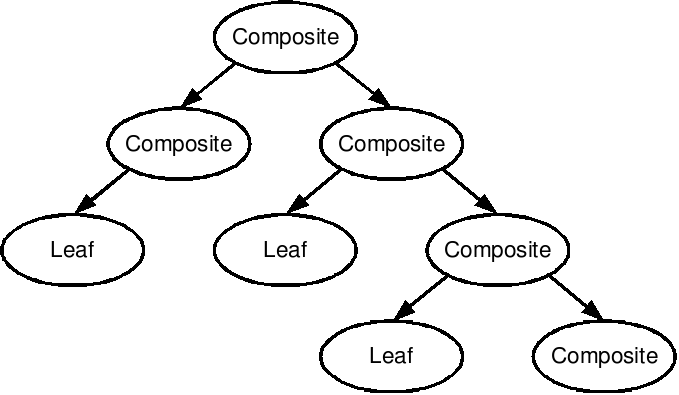
\includegraphics[scale=0.45]{Figures/modeling_notions/composite_tree.png}
    \caption{Example of tree modeled by the Composite.}\label{fig:composite_tree}
  \end{center}
\end{figure}

The Composite pattern is an essential element of the design model for the \OT\ platform. It can be used to model numerical function composition, random vector composition, etc. It can be found in several aspects of the modeling brick. Any related objects tree structure can rely on the Composite pattern with benefit.

\label{iterator}\subsection{Iterator pattern}

The role of this pattern is to provide a means of sequentially accessing elements of a collection or of an aggregate, without breaking the encapsulation principle that forbids to expose the collection's underlying implementation. For an iterator to be able to access the elements of an aggregate encapsulating its internal representation, it must have privileged access. Figure \ref{fig:iterator} illustrates this pattern.

\begin{figure}[htb]
  \begin{center}
    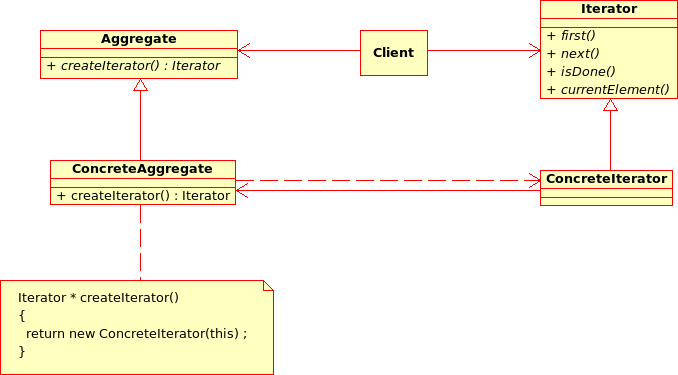
\includegraphics[scale=0.5]{Figures/modeling_notions/iterator.png}
    \caption{Iterator structure.}\label{fig:iterator}
  \end{center}
\end{figure}

The iterator is jointly used with the Composite pattern to traverse trees relying on internal objects (vectors, functions, etc.).

\label{visitor}\subsection{Visitor pattern}

The Visitor pattern allows to conduct a given operation on a hierarchy of objects without changing the classes of these objects. The processing is supported by the Visitor which moves from one object to another and applies the correct treatment on each object according to its class. By changing the Visitor, we can therefore apply different treatments. The class hierarchy must not substantially evolve through these operations.

Figure \ref{fig:visitor} illustrates the twofold class hierarchy of Nodes and Visitors which are orthogonal (contrary to the Factory in which they are parallel): the Visitor has as many methods are there are Nodes in the hierarchy.

\begin{figure}[htb]
  \begin{center}
    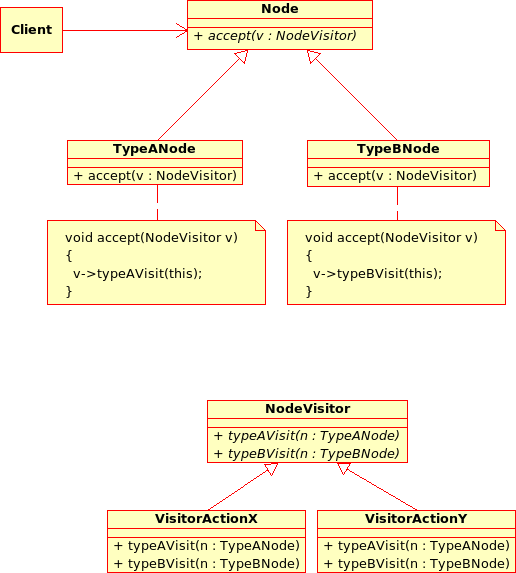
\includegraphics[scale=0.5]{Figures/modeling_notions/visitor.png}
    \caption{Visitor structure.}\label{fig:visitor}
  \end{center}
\end{figure}

As far as the client is concerned, the processing is limited to instantiating a Visitor of the right type and applying it to the class hierarchy.. The Visitor pattern is often jointly used with the Composite pattern (to model object trees) and with the Iterator pattern (to traverse the collection of objects).

The Visitor can be used within the \OT\ platform to conduct global operations on the trees representing composite functions (e.g. for derivation), on random vectors (to save them or evaluate a realization or a sample), etc.

\section{Package description}

In this section, we begin the study of the classes and objects developed for the \OT\ platform. The definitions given here are those implemented in the tool's final code. Contrary to the analytical approach (which aimed at viewing the platform's constituting elements from a functional and more general point of view), this chapter adopts a development oriented point of view. We shall begin with the lowest layers of the system and move up to the top-level ones.

The reader may find symbols symbols made up of a name followed by two colons (::): it designates a namespace as described in section \ref{namespace}. For example, OT:: designates the namespace called OT.

All of the elements developed for the \OT\ platform belong to an OT namespace.

\emph{NB: Very often, the class definitions indicate that the values used to create an object cannot be modified once the object is created. This conservative mechanism was intentionally adopted in the early stages of development so as to narrow the object's interface and to simplify the mechanisms handling dependencies between objects. However, this may prejudice the ergonomy of the platform. Shall this decision cause problems, the constraint can be lifted. It would then only require to add the appropriate methods to the object's interface, which is easier to handle than withdrawing methods already implemented.}

\subsection{Basis brick}

This encompasses all of the classes supporting the field-specific brick, which means the programming classes associated with the language or the implementation, as well as the classes offering elementary functions associated with the field-specific aspects of the platform.

\subsubsection{Data types}

The source files of these bricks are stored in the Base/Type subfolder of the source tree.

\label{id}\paragraph{Id}

The Id is a \emph{unique} identifier for each object instantiated by the \OT\ platform. Unicity is guaranteed at the level of a study but not between different studies. The identifier must be compact so as not to weigh down on the objects (especially the smaller ones) and it must be generated quickly so as to not substantially slow down the object creation. It is thus preferable to associate it with an elementary type of the language, for example an \emph{unsigned long}. Moreover, it must support a weak order relation (operator \textless) and a comparison relation (operators == and !=) so that it can be used as a key in a container.

Not all objects possess an Id: only those which need to be persistent have one. Therefore temporary objects, volatile objects and any object that can be re-created from its value carry no Id. By default, an object which can be backed up in a study has an Id.

When re-creating a backed up object that had an Id, the Id is restored to its value prior to the backup: this means that the Id is saved within the object in the study.

\paragraph{NumericalScalar}

In its standard version, the \OT\ platform only performs computations on real numbers. Future versions may include other numerical types.

This type of real numbers is designated as NumericalScalar and must be able to store any floating point number. Thus the NumericalScalar type is associated with the \emph{double} type of the programming language.

\paragraph{String}

So as to provide the user with a means of naming the objects they are handling according to the current study, the platform will use a type allowing to store character strings of any length and encoding type (see \cite{UNICODE}).

Please note that this type is not appropriate for naming files, directories, URL, etc. For more details on this, refer to the FileName type described in next section.

The String type is associated with the std::string type from the C++ STL (see \cite{C++} and \cite{EffSTL}). It depends on the locale setting of the user.

\paragraph{FileName}

The FileName type differs from the String type in that it is meant to store the names of files, directories, URLs, etc., not any type of word the user might need. The names stored in a FileName object have to be interpretable on the computer executing the \OT\ platform. The character set of the encoding system used by FileName may be more limited than that of String.

The FileName type is associated with the std::string type from the C++ STL (see \cite{C++} and \cite{EffSTL}).

\paragraph{Bool}

In order to store or return a boolean value, the platform uses the Bool type. The Bool type is based on the standard C++ bool type.

\paragraph{UnsignedLong}

In order to store natural numbers, the platform uses the UnsignedLong type. This type appears everywhere where a collection or table size, an index, a quantity, etc. are involved.

It can be derived into more specialized sub-types such as Size, Index, etc.

The UnsignedLong type is programmed as an \emph{unsigned long}.

\paragraph{LibraryHandle}

In order to store or return a handle for a loaded dynamic library, the platform uses the LibraryHandle type. The LibraryHandle type is based on the standard C++ void * type.

\paragraph{LibrarySymbol}

In order to store or return an identifier for a symbol belonging to a library, the platform uses the LibrarySymbol type. The LibrarySymbol type is based on the standard C++ void * type.

\subsubsection{Common classes}

The common classes are programming objects used to support more elaborate classes. They are meant to provide common services for all objects handled in the platform. The source files of these classes are in the Base/Common sub-folder of the source tree.

\paragraph{Object}

The vast majority of objects instantiated in the \OT\ platform derive from the Object class.

This abstract class (described in Figure \ref{fig:obj} provides support for the object's name \emph{name\_}. It can also be used to implement other global properties for the objects, which will be defined in future versions of the platform.

The object's name can be accessed with the \emph{setName()} and \emph{getName()} methods. \emph{Neither one of these methods is virtual, thus they cannot be redefined}.

The object's name is passed to the Object class constructor. The default value for the object's name is the constant value: Unnamed.

\begin{figure}[htb]
  \begin{center}
    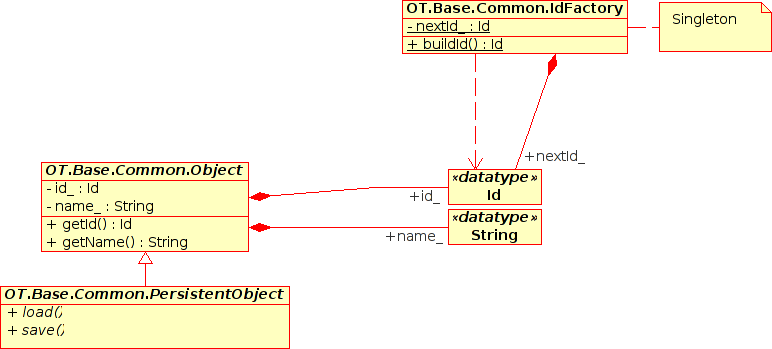
\includegraphics[scale=0.5]{Figures/design/Object.png}
    \caption{Object, PersistentObject and IdFactory classes.}\label{fig:obj}
  \end{center}
\end{figure}

The Object class also provides a virtual method \emph{str()} which allows any instance deriving from Object to be displayed as a stream. Each class deriving from Object must overdefine this method.

The Object class defines a comparison operator \emph{operator ==()} which tests if the values of two objects are equal. Note that this is different from an identity test (which is defined in the PersistentObject class).

\paragraph{PersistentObject}

The PersistentObject class is a specialization of Object which provides backup and restore services for the objects based on a stream (std::stream). This stream can be connected to a file, a socket, etc. It is described in Figure \ref{fig:obj}.

It offers a \emph{load()} method which allows to re-read an object from the stream, and a \emph{save()} method to write the object in the stream. Both methods are pure virtual methods and thus they will have to be redefined in the derived classes. The stream handling mode on which the reading and writing will be based on is not defined yet: method arguments, global object, study related object, etc. are different possibilities that currently still need to be studied.

This class also defines an id\_\ ~attribute which contains a unique identifier for the object. This identifier is automatically assigned when the object is created and it cannot be redefined. It is a read-only attribute that can be accessed with the \emph{getId()} method. The identity of two objects can be tested with the \emph{is()} method, which returns a \emph{true} boolean value if both objects are identical.

\paragraph{IdFactory}

The IdFactory is a factory (see section \ref{factory}) which produces a unique identifier Id each time its \emph{buildId()} is invoked. It is at the IdFactory level that the unicity and sequentiality of the Ids are handled. The IdFactory must be unique so as to prevent generating several identical Ids. This object must therefore implement the Singleton design pattern (see section \ref{singleton}). The rules that govern the Ids (see section \ref{id}) imply that this singleton is managed at the study level.

The IdFactory is described in Figure \ref{fig:obj}.

\paragraph{Exception}

Unless in duly justified and allowed cases, any error detected within the \OT\ platform is brought all the way up to the user level through exceptions. The Exception class, which derives from std::exception, is the mother class to all of the platform's exceptions. It is forbidden to develop an exception class which would not derive from Exception.

Exception and all of its sub-classes must redefine the methods of std::exception. The Exception class is described in Figure \ref{fig:exception}.

\begin{figure}[htb]
  \begin{center}
    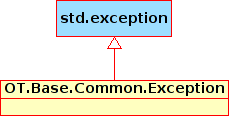
\includegraphics[scale=0.5]{Figures/design/Exception.png}
    \caption{Exception class.}\label{fig:exception}
  \end{center}
\end{figure}

Exception can be derived into various sub-classes such as:
\begin{enumerate}
\item FileNotFoundException
\item InvalidArgumentException
\item NoWrapperFileFoundException
\item WrapperFileParsingException
\item WrapperInternalException
\item XMLException
\item XMLParserException
\item DynamicLibraryException
\item etc.
\end{enumerate}

\paragraph{FileNotFoundException}
This exception is raised when a file required by the platform is not found.

\paragraph{InvalidArgumentException}
This exception is raised when an argument passed to a method is incorrect and prevents the method from following its usual course of actions.

\paragraph{NoWrapperFileFoundException}
This exception is raised when the wrapper description file cannot be found.

\paragraph{WrapperFileParsingException}
This exception is raised when an error is detected in the wrapper description file, which prevents the file parsing.

\paragraph{WrapperInternalException}
This exception is raised when a fatal error occurs in the wrapper or one of its methods.

\paragraph{XMLException}
This exception is raised when an error occurs during the XML description file's parsing.

\paragraph{XMLParserException}
This exception is raised when the XML parser for the description file detects an internal error.

\paragraph{DynamicLibraryException}
This exception is raised when an error is detected while loading or unloading one of the platform's dynamic libraries.

\paragraph{Iterator}

The Iterator class is the abstract class from which all iterator classes derive. As described in Figure \ref{fig:iterator}, the Iterator defines the following pure virtual methods:
\begin{itemize}
\item \emph{begin()} to point at the beginning of the collection;
\item \emph{end()} to point at the end of the collection;
\item \emph{more()} to determine if there are any elements in the collection that were not reached yet;
\item \emph{currentElement()} to access the element currently pointed at in the collection by the iterator.
\end{itemize}

These methods must be re-defined by Iterator's sub-classes. Iterator only defines an interface.

\paragraph{Pointer}
Figure \ref{fig:pointer} describes the Pointer class as using the BOOST shared\_ptr class (see \cite{BOOST}). It is a \emph{smart pointer} supporting copy construction and assignment. The ownership of the object is shared by all of Pointer's instances pointing at it and the last pointer is in charge of deleting the object.

The use of the Pointer class allows to noticeably reduce the platform's memory consumption and enhances its performance since it prevents useless object copy operations and costly memory allocations. In return, however, this requires a subtle management of the objects and a careful study of their life-cycle within the platform: deleting the pointer does not ensure that the object itself is deleted, since the object ownership may have been transfered to another pointer. \emph{More specifically, the use of Pointer de facto forbids the use of C++ classic pointers. The only exception to this rule is the parameter transfer between the platform and the wrapper, since the API is written in C.}

The Pointer class is a template: there will have to be as many specialized Pointer classes as there are classes subject to this mechanism. A naming convention will be described in \cite{OT} so that the pointer's name can be deduced from the class name.

\begin{figure}[htb]
  \begin{center}
    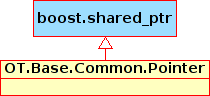
\includegraphics[scale=0.5]{Figures/design/SharedPointer.png}
    \caption{Pointer class.}\label{fig:pointer}
  \end{center}
\end{figure}

The Pointer class offers the following services:
\begin{itemize}
\item constructors and destructors respectively support and delete the object pointed at;
\item the assignment operator \emph{operator =()} and the copy constructor transfer and share responsibility for the object;
\item the \emph{reset()} method replaces the object pointed at;
\item the operators \emph{operator *()} and \emph{operator -\textgreater()} give access to the object pointed at;
\item the \emph{swap()} method allows to swap objects pointed at by two pointers;
\item the \emph{unique()} method allows to check if the pointer is the object's sole owner;
\item the \emph{use\_count()} method allows to check the number of owners for the object pointed at.
\end{itemize}

By default, the Pointer class uses the BoostPointerImplementation class for its implementation. This choice can be re-defined when using the Pointer class by passing the name of the implementation class as a second argument for the template. In the initial version of the \OT\ platform, only the BoostPointerImplementation class will be offered.

\paragraph{BoostPointerImplementation}
This class represents a shared pointer based on the BOOST library (see \cite{BOOST}). It is used through the Pointer class.

\paragraph{Thread}

The \OT\ platform is designed to launch and control computations that can take quite some time. The general ergonomy implies that the user remains in control of the tool during these costly operations. It is thus necessary to provide a mechanism to launch computations asynchronously, based, for example, on threads (see \cite{Thr}). The Thread class, which is described in Figure \ref{fig:threadable}, implements this mechanism.
A Thread object is created with the support of a Threadable object encapsulating the computation to be carried out. The execution itself starts when the object's \emph{run()} method is called. This method then launches the Threadable object's \emph{run()}. The \emph{run()} method of the Thread object is asynchronous: it immediatly returns and the execution of the programm goes on parallelly to the computation. This method may raise exceptions if the computation launch fails for any reason.

The Thread object can be interrogated with the \emph{query()} to know the computation's progress.

The \emph{wait()} method is used to wait for the computation to terminate. It sets a lock until the computation terminates. It returns if the computation terminates in a normal or abnormal state. In the latter case, an exception is propagated if it was emitted by the computation.

\begin{figure}[htb]
  \begin{center}
    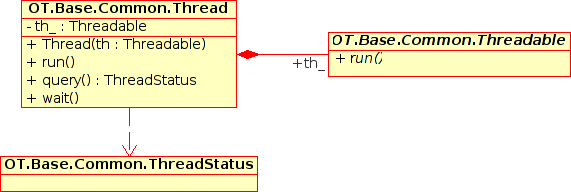
\includegraphics[scale=0.5]{Figures/design/Threadable.png}
    \caption{Thread, Threadable and ThreadStatus classes.}\label{fig:threadable}
  \end{center}
\end{figure}

\paragraph{ThreadStatus}
The \emph{query()} method of the Thread class returns a ThreadStatus object which gives access to information about the computation's course: its state (running, terminated, stopped, etc.), its progress (x\% computed), etc.

Details about ThreadStatus methods will be given in a future version of this document.

\paragraph{Threadable}

The Threadable class is an abstract class defining an interface for all classes which can be passed as arguments to a Thread object. It defines a pure virtual \emph{run()} method which will have to be re-defined in sub-classes.

This \emph{run()} method must execute the computation implemented by the class.

Though not defined here yet, the Threadable class must provide a means of communicating with the Thread class, so as to notify if of the computation's state and progress. This way, the Thread class can in turn relay this information to the user.

\paragraph{Lockable / Lock}

The abstract Lockable class defines an interface for the derived classes. All of the classes used in a multithreaded environment (which will have to support concurrent access from several threads) must derive from Lockable.

Lockable defines a sub-class Lock which sets up a limited scope locking mechanism. The definition of a lock on the object deriving from Lockable helps ensuring the serialization of the block in which this lock is defined. This mechanism allows to easily declare critical sections without having to worry about the lock's lifespan or its release.

\paragraph{Path}

Path is a non-instantiable class which defines static methods to search through the computer's filesystem tree. These methods implement algorithms that are common to all classes of the platform needing them. Thus all mechanisms are gathered in a single and well identified structure, which makes the maintenance easer.

The static \emph{GetDirectoryList()} returns the list of directories in which the search must be conducted. The returned object is a list of directories which can be modified.

The static \emph{FindFileByNameInDirectoryList()} returns the full path to the first file whose name is passed as an argument, in the directory list also passed as an argument. The function simply searches the filesystem. It does not provide any locking mechanism or any sort of preemption on the file, which means that the file can have disappeared or changed names when the result of \emph{FindFileByNameInDirectoryList()} is actually used.

\paragraph{StorageManager}

This abstract class defines an interface for all of the storage managers handling data on the filesystem. It defines the methods that any instantiable manager must provide.

A StorageManager browses through all of the PersistentObjects and saves them on the filesystem. Conversely, a StorageManager can restore saved PersistentObjects to their prior saving state without any noticeable change in the application's execution once the data is reloaded.

\paragraph{WrapperFile}

The WrapperFile class offers a means of handling the description file for an external code wrapper. The class constructor allows to read the file in the filesystem. Once the file has been read and parsed, the class data structures are updated with the file's descriptive elements.

The class offers a set of accessors to update and retrieve the data read in the description file.

It also provides a static \emph{FindWrapperPathByName()} method which relies on the Path class to search the file in the filesystem.

Depending on how the platform's code is compiled, the WrapperFile class allows to read and parse files in different formats: XML, plain text, etc. Depending on the case, the class calls the appropriate parser which may have been included in the platform.

\paragraph{WrapperData}

This structure stores the data that can be exchanged between the wrapper and the \OT\ platform. This data is read in the wrapper's description file and stored in a WrapperFile object. It can be accessed through the \emph{getWrapperData()} method of the WrapperFile object.

The WrapperData class allows access to the list of the wrapper's input and output files with the \emph{getFileList()} method. The list of variables to be substituted in these files can be accessed with \emph{getVariableList()}.

This data cannot be directly transferred to the wrapper, whose interface is written in C. Therefore, equivalent methods are provided to return this information as a C chained list. These methods are respectively known as \emph{getNewFileListForCInterface()} and \emph{getNewVariableListForCInterface()}. As their name indicates, these methods dynamically allocate the objects, which will thus have to be deallocated once they become useless. To achieve this, two methods are provided, namely \emph{freeFileListForCInterface()} and \emph{freeVariableListForCInterface()}. Though the data is sent to the wrapper, it is not up to the wrapper to ensure that the memory is deallocated. It is therefore up to the wrapper's caller to create and free the appropriate memory space.

\paragraph{XMLStringConverter}

When an XML parser is used, it is necessary to convert character strings read in the file by the parser into String elements. This conversion is the reason why the XMLStringConverter class exists. The constructor reads the XML string and the operator \emph{operator String()} converts it into a String.

\paragraph{XMLWrapperErrorHandler}

This class allows to implement an error handler for the XML parser integrated in the \OT\ platform. The parser automatically invokes it when an error occurs, to ensure that the error is correctly handled.

\subsubsection{Base type}

The base types of the \OT\ platform are grouped into a package which corresponds to classes stored in the Base/Type sub-folder of the source tree. This package includes higher level classes which have a meaning in the context of statistics. They will be the foundation for the definition of the tool's data model.

\paragraph{Collection}
Figure \ref{fig:collection} shows the definition of the Collection class as a class deriving from std::vector. The Collection represents an ordered set of homogeneous objects. Thus an iterator can traverse it, the user can interrogate its size, elements can be added or removed, etc.

As the std::vector type, the Collection class is a template that will have to be instantiated with the collection's element type. Figure \ref{fig:collection} shows a DistributionCollection sub-class instantiated with the Distribution type.

\begin{figure}[htb]
  \begin{center}
    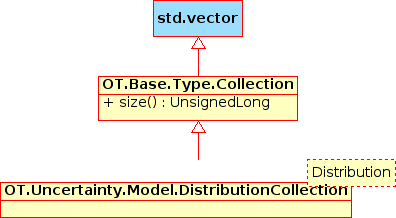
\includegraphics[scale=0.5]{Figures/design/Collection.png}
    \caption{Collection and DistributionCollection classes.}\label{fig:collection}
  \end{center}
\end{figure}

\paragraph{NumericalPoint}

The NumericalPoint class implements the notion of numerical point. It is an ordered collection of numerical scalars representing the coordinates of a point in a space of any given dimension ($\Re^{n}$), where n is the point's dimension. NumericalPoint's \emph{dim()} method returns this dimension. \emph{Note that NumericalPoint does not inherit the size() method from Collection}. Neither can a NumericalPoint's dimension be modified the way a Collection's size attribute can. A NumericalPoint's dimension is defined once and for all when the object is created.

\begin{figure}[htb]
  \begin{center}
    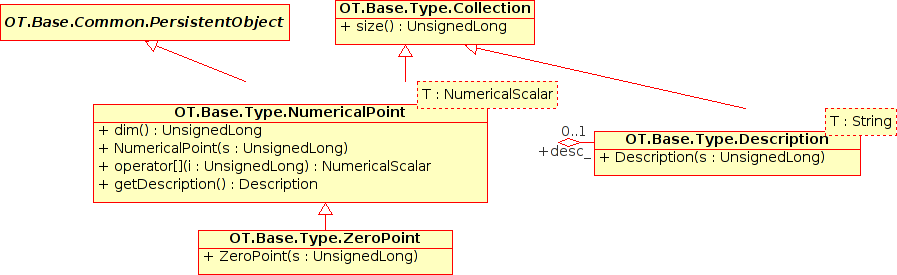
\includegraphics[scale=0.5]{Figures/design/NumericalPoint.png}
    \caption{Collection, NumericalPoint, ZeroPoint and Description classes.}\label{fig:numpoint}
  \end{center}
\end{figure}

The operator \emph{operator[]()} is provided to access the NumericalPoint's coordinates. It returns a reference to the coordinate.

The \emph{getNorm()} method returns the point's norm.

The NumericalPoint can be associated to a Description which has mandatorily the same size and details each coordinate, for example by associating it with a meaningful name for the user. It can also have a specific name provided by the PersistentObject class from which it inherits.

\paragraph{ZeroPoint}

The origin point playing a distinctive and recurring role in modeling, a specific class is created to represent it and accelerate computations. Functionnally speaking, it is a NumericalPoint; however, all of its coordinates have a zero value and they cannot be modified.

\paragraph{Description}
The Description is a String collection which can be associated to any object of a multi-dimensional nature. It allows to describe the components of the entity it is associated with by giving each one a name (or a comment, etc.) that is meaningful for the platform user. No processing can be carried out on the basis of the description which is only available for informative purposes.

However, Descriptions can be shared between objects of the same nature: for example, all of the NumericalPoints of a given sample and the sample itself may use the same Description.

\begin{figure}[htb]
  \begin{center}
    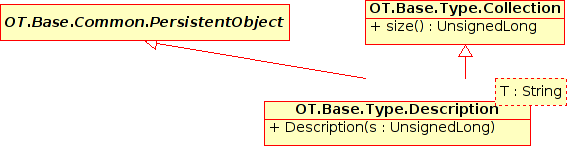
\includegraphics[scale=0.5]{Figures/design/Description.png}
    \caption{Collection and Description classes.}\label{fig:description}
  \end{center}
\end{figure}

\paragraph{Matrix}
The Matrix class (see Figure \ref{fig:mat}) implements the notion of numerical scalar matrix, which is a two-dimensional ordered Collection of NumericalScalars. Its size is fixed when the object is created and it cannot be modified later on. The \emph{getNbRows()} and \emph{getNbColumns()} methods respectively return the matrix's number of rows and its number of columns.

As in all matrices, the operator \emph{operator()} gives access to the numerical scalar designated by the row and column indexes passed as arguments.

The \emph{transpose()} method returns the transposed matrix of the original matrix.

\begin{figure}[htb]
  \begin{center}
    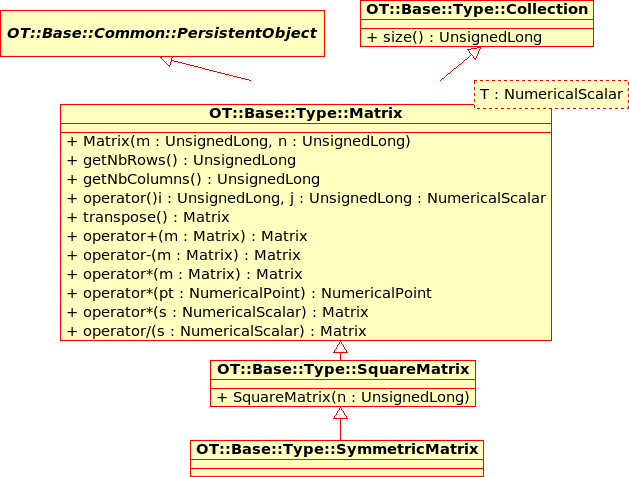
\includegraphics[scale=0.5]{Figures/design/Matrix.png}
    \caption{Collection, Matrix, SquareMatrix and SymmetricalMatrix classes.}\label{fig:mat}
  \end{center}
\end{figure}

The Matrix class supports an elementary algebra for which the following operations are defined: addition and substraction (with another Matrix), product (with another Matrix, with a NumericalPoint, with a NumericalScalar), division (with a NumericalScalar). The set of algebraic operations may be extended later on. These operations all rely on the underlying external library LAPACK.

\paragraph{SquareMatrix}

The SquareMatrix class derives from Matrix and restricts the behavior of the Matrix class to the case of square matrices. Specifically, the SquareMatrix constructor only accepts one argument.

\paragraph{SymmetricMatrix}

As described in Figures \ref{fig:mat} and \ref{fig:symmatrix}, the SymmetricMatrix class specializes SquareMatrix for the symmetric matrices. Specifically, the operator \emph{operator()} is implemented so as to compel the user to create a symmetric matrix: the matrix is stored in an upper triangular form, and only the elements above the diagonal are read or modified. This ensures that the matrix is constantly consistent with its definition.

\begin{figure}[htb]
  \begin{center}
    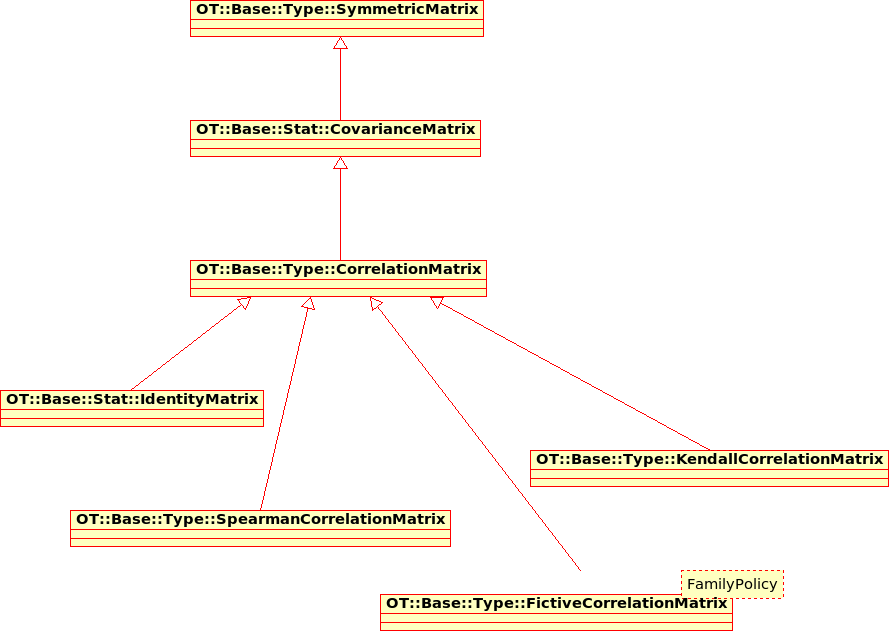
\includegraphics[scale=0.45]{Figures/design/SymmetricMatrix.png}
    \caption{SymmetricMatrix, CovarianceMatrix, IdentityMatrix, CorrelationMatrix, and related classes.}\label{fig:symmatrix}
  \end{center}
\end{figure}

\paragraph{CorrelationMatrix}

The CorrelationMatrix class specializes SymmetricMatrix for the correlation matrices. The distinctive definition rules for these matrices require a specific method to ensure that, if modified, the matrix elements' values still obey these rules: the value of the diagonal elements must always be 1, the value of non-diagonal elements belong to the [$-$1, 1] interval, etc.

\paragraph{FictiveCorrelationMatrix}

The FictiveCorrelationMatrix is a template class deriving from CorrelationMatrix, whose constructor implements mechanisms to convert different types of correlation matrices (KendallCorrelationMatrix, SpearmanCorrelationMatrix, etc.) into a fictive correlation matrix. The conversion mechanism is defined in a FamilyPolicy class.

\paragraph{KendallCorrelationMatrix}

The KendallCorrelationMatrix class is a CorrelationMatrix whose coefficients are Kendall correlation coefficients. This class will be developed in a future version of the platform.

\paragraph{SpearmanCorrelationMatrix}
The SpearmanCorrelationMatrix class is a CorrelationMatrix whose coefficients are Spearman correlation coefficients. This class will be developed in a future version of the platform.

\paragraph{Tensor}

The Tensor class described in Figure \ref{fig:tensor} is a three dimensional ordered collection of numerical scalars. It implements the concept of mathematical tensor. To this date, no algebra is defined on this class.

\begin{figure}[htb]
  \begin{center}
    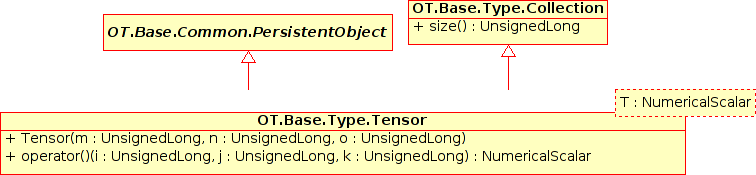
\includegraphics[scale=0.5]{Figures/design/Tensor.png}
    \caption{Collection and Tensor classes.}\label{fig:tensor}
  \end{center}
\end{figure}

\paragraph{FamilyPolicy}

Figure \ref{fig:fampol} describes the abstract FamilyPolicy class which defines an interface for all of the correlation matrix conversions. It is implemented as a template instantiated for each conversion operating on a pair of correlation matrices.

\begin{figure}[htb]
  \begin{center}
    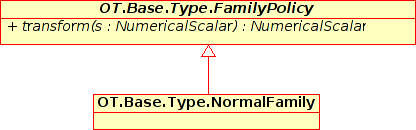
\includegraphics[scale=0.5]{Figures/design/FamilyPolicy.png}
    \caption{FamilyPolicy and NormalFamily classes.}\label{fig:fampol}
  \end{center}
\end{figure}

The \emph{transform()} is applied element by element on the intial matrix to produce the final matrix (generally a fictive matrix).

\paragraph{NormalFamily}
The NormalFamily class specializes the FamilyPolicy class for Gaussian fictive matrices. It implements several definitions for the \emph{transform()} method depending on the original matrix.

\subsubsection{Basic numerical functions}

This package encompasses classes implementing all of the mechanisms linked to the numerical functions of the \OT\ platform.

These elements are grouped in the Base/Func sub-folder of the source tree.

\paragraph{NumericalMathFunction}
The \OT\ platform offers a definition for the numerical function (on this subject, refer to section \ref{numericalfunction}) implemented as a class called NumericalMathFunction. It is an abstract class, thus defining a common interface for all of the tool's numerical functions. Therefore, it is derived into several sub-classes implementing different types of functions (see Figure \ref{fig:nummathfun} and the following paragraphs).

The NumericalMathFunction class defines a pure virtual operator \emph{operator()} which returns the result of the function call for a given point.

The NumericalMathFunction can be interrogated to retrieve the numerical point dimentions used for input and output with the \emph{inNumericalPointDim()} and \emph{outNumericalPointDim()}.

The pure virtual methods \emph{gradient()} and \emph{hessian()} respectively return the function's gradient matrix and hessian tensor at the given point.

\begin{figure}[htb]
  \begin{center}
    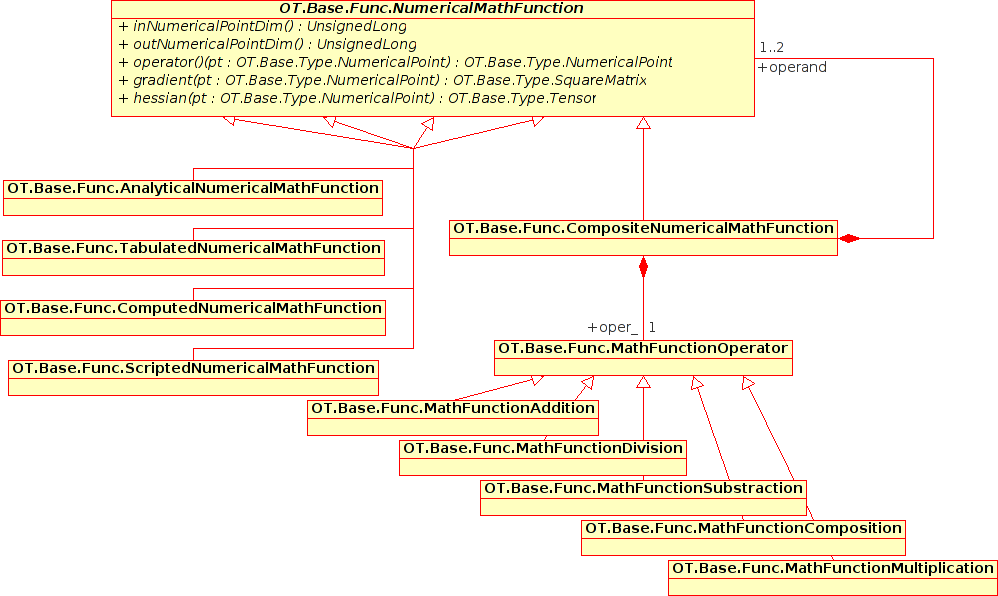
\includegraphics[scale=0.4]{Figures/design/NumericalMathFunction.png}
    \caption{NumericalMathFunction and related classes, MathFunctionOperator and related classes.}\label{fig:nummathfun}
  \end{center}
\end{figure}

\paragraph{AnalyticalNumericalMathFunction}

The AnalyticalNumericalMathFunction class derives from NumericalMathFunction and implements an analytical function directly coded in the \OT\ platform.

Among these functions can be found all of the standard mathematical functions whose analytical expression as well as its gradient and hessian are known, commonly used in uncertainty treatment studies (e.g. $\sin$, $\cos$, $\exp$, etc.).

\paragraph{TabulatedNumericalMathFunction}
The TabulatedNumericalMathFunction class derives from NumericalMathFunction and implements a function whose values are known only for given intervals, generally in an empirical fashion. This type of function is designed either to have its values directly created by the user through the platform's GUI or to be read from a description file.

The values taken by the function are given as a collection of values when the object is created and they cannot be modified later on. It is conceivable to design a factory allowing to create such functions by reading a stream using different formats.

\paragraph{ComputedNumericalMathFunction}
The ComputedNumericalMathFunction class derives from NumericalMathFunction and represents a function implemented within a compiled code linked to the \OT\ platform. It is here that the connection with external code occurs and the ComputedNumericalFunction class virtualizes the external code into a mathematical function.

The external code is not directly linked to the ComputedNumericalMathFunction operator \emph{operator()} but rather to an intermediary object that establishes the programming link between the code and the mathematical function.

\paragraph{ScriptedNumericalMathFunction}
The ScriptedNumericalMathFunction class derives from NumericalMathFunction and represents a function implemented within the integrated Python interpreter of the \OT\ platform. This function can be called as well from the Python interpreter in which it is defined as from the C++ code, yet without offering the same performance level as a C++ coded function.

\paragraph{CompositeNumericalMathFunction}

The \OT\ platform intends to provide for the combination of numerical functions with an elementary algebra allowing to add, substract, multiply, divide and compose numerical functions. The CompositeNumericalMathFunction class is where this combination takes place. It points to one or two numerical functions (type NumericalMathFunction) which behave as operands and play symmetric or dissymmetric roles (depending on the operation). Figure \ref{fig:nummathfun} clearly shows the Composite design pattern (see section \ref{composite}) where the AnalyticalNumericalMathFunction, TabulatedNumericalMathFunction, ComputedNumericalMathFunction, etc. classes represent the tree's leaves.

With this Composite pattern, it is possible to represent any combination of functions linked with unary or binary operators. This mechanism allows to set up chains of external codes within the \OT\ platform.

\paragraph{MathFunctionOperator}
Figure \ref{fig:nummathfun} shows that the CompositeNumericalMathFunction class is related to an abstract MathFunctionOperator class representing the operator to be applied on the combination of numerical functions. This operator must be derived into sub-classes actually implementing the expected combinations.

\paragraph{MathFunctionAddition}
The MathFunctionAddition class derives from MathFunctionOperator and implements the sum of two numerical functions. It checks that both numerical functions return NumericalPoints of the same dimension, and raises an exception if it is not the case when creating the CompositeNumericalMathFunction object.

\paragraph{MathFunctionSubstraction}
The MathFunctionSubstraction class derives from MathFunctionOperator and implements the substraction of two numerical functions. It checks that both numerical functions return NumericalPoints of the same dimension, and raises an exception if it is not the case when creating the CompositeNumericalMathFunction object.

\paragraph{MathFunctionMultiplication}
The MathFunctionMultiplication class derives from MathFunctionOperator and implements the product of a numerical function by a numerical scalar (NumericalScalar).

\paragraph{MathFunctionDivision}
The MathFunctionDivision class derives from MathFunctionOperator and implements the division of a numerical function by a numerical scalar (NumericalScalar). It raises an exception in case of a division by zero when invoking the function or one of its methods.

\paragraph{MathFunctionComposition}
The MathFunctionComposition class derives from MathFunctionOperator and implements the composition of two numerical functions. It checks that both numerical functions return / uses NumericalPoints of compatible dimensions, and raises an exception if it is not the case when creating the CompositeNumericalMathFunction object.

\paragraph{Library}
This class abstracts access to dynamic libraries loaded in the platform by hiding the operations into an object. The Library object thus retains the reference to the dynamic library and allows to search for symbols exported by this library with the \emph{getSymbol()} method.

Objects from the Library class cannot be directly instantiated. They are created by a LibraryLoader object.

\paragraph{LibraryLoader}
The LibraryLoader class provides a factory mechanism to produce Library objects. The LibraryLoader class also provides a singleton mechanism through the \emph{getInstance()} static method. Once the LibraryLoader object is retrieved, it is possible to load a library with its \emph{load()}. This method returns a Library object representing the library, which allows access to the symbols exported by the library.

The LibraryLoader object is multithread-safe.

\paragraph{NumericalWrapperFunction}
The NumericalWrapperFunction class implements general mechanisms allowing the use of an external wrapper for access to a numerical function located in an external code. Access to the wrapper relies on a loaded dynamic library.

Since the wrapper can be called concurrently by the platform, a state management mechanism must be provided and the state needs to be stored in the ComputedNumericalMathFunction object. This state, whose internal representation is specific to the wrapper, can be accessed through the \emph{createNewState()} and \emph{deleteState()} methods. It is entirely handled by the ComputedNumericalMathFunction object.

The NumericalWrapperFunction object defines an interface to access the wrapper with the following pure virtual methods:
\begin{itemize}
\item \emph{getInNumericalPointDimension()}: access to the dimension of the function's input vector;
\item \emph{getOutNumericalPointDimension()}: access to the dimension of the function's output vector;
\item \emph{initialize()}: initializes the wrapper before the first access to the function occurs;
\item \emph{execute()}: executes the external code function: the input vector is passed to the function and the output vector is retrieved;
\item \emph{finalize()}: finalizes the wrapper after the last access to the function occurs.
\end{itemize}

The NumericalWrapperFunction object is built based on the path to a library, a symbol anme and initialization data for the wrapper. Parsing the wrapper's description file (cf. WrapperFile et WrapperData) provides all of the necessary data.

\paragraph{UsualNumericalWrapperFunction}
The UsualNumericalWrapperFunction class derives from NumericalWrapperFunction and implements the interface it defines, namely the getInNumericalPointDimension(), getOutNumericalPointDimension(), initialize(), execute() and finalize() methods.

\subsubsection{Statistical objects}

This package encompasses classes offering higher-level statistical functionalities in the \OT\ platform. This package integrates notions such as numerical sample, covariance matrix, etc.

These elements are grouped into the Base/Stat sub-folder of the source tree.

\paragraph{CovarianceMatrix}
The CovarianceMatrix class, described in Figure \ref{fig:symmatrix}, specializes SymmetricMatrix for covariance matrices.

\paragraph{IdentityMatrix}
The Identity matrix playing a distinctive, recurrent role in modeling, it is associated to a specific class IdentityMatrix in order to improve performance. From a functional point of vew, it is a SymmetricMatrix; the value of its diagonal elements is 1, the value of its non-diagonal elements is 0, and the elements cannot be modified.

\paragraph{NumericalSample}
The NumericalSample class described in Figure \ref{fig:numsample} is an abstract class representing a one-dimensional ordered collection of numerical points (NumericalPoint objects). Thus it defines an interface for all of the classes deriving from it.

\begin{figure}[htb]
  \begin{center}
    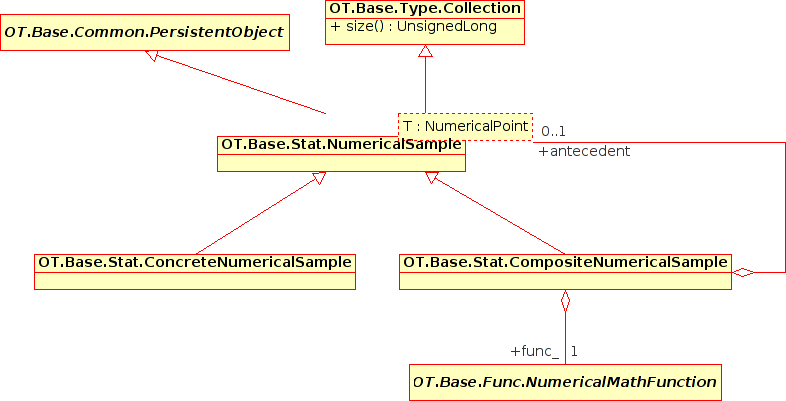
\includegraphics[scale=0.5]{Figures/design/NumericalSample.png}
    \caption{Collection, NumericalSample, and related classes.}\label{fig:numsample}
  \end{center}
\end{figure}

Objects from the NumericalSample class provide a pure virtual \emph{getMeanValue()} which returns a numerical point giving the mean value of the sample's points.

The pure virtual method \emph{getCovariance()} returns the sample's covariance matrix.

The operator \emph{operator()} gives access to the sample's individual points.

Figure \ref{fig:numsample} shows that the NumericalSample class matches a Composite design pattern as described in section \ref{composite}.

\paragraph{ConcreteNumericalSample}
The ConcreteNumericalSample represents a leaf in the Composite pattern. It derives from the abstract class NumericalSample and defines instantiable samples on which it is possible to carry out statistical treatments.

Points can be added or removed from the collection with both methods \emph{add()} and \emph{remove()}. It is the standard way for the user to handle the sample's content.

\paragraph{CompositeNumericalSample}
The CompositeNumericalSample class derives from the abstract NumericalSample class and defines a sample whose elements are based on another sample and a numerical function (NumericalMathFunction). It takes part in the implementation of a Composite pattern and sets up the chain between numerical samples.

When a CompositeNumericalSample is created, the collection contains no element. These are determined on demand when methods are applied to the sample. They result from the call of the numerical function on the elements of the antecedent sample. Since the amount of elements can be very high, it is compulsory to consider a parallel processing of the calls within the CompositeNumericalSample class.

\paragraph{NumericalSampleFactory}
The content of a numerical sample can be directly provided by a file, a stream, etc. These possibilities are not directly cared for by objects from the NumericalSample class by a distinct class hierarchy of NumericalSampleFactory objects implementing a Factory pattern (see section \ref{factory}).

\begin{figure}[htb]
  \begin{center}
    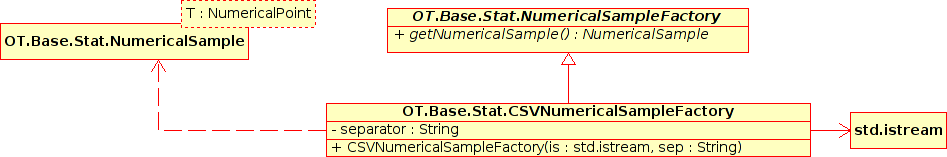
\includegraphics[scale=0.5]{Figures/design/NumericalSampleFactory.png}
    \caption{NumericalSampleFactory, CSVNumericalSampleFactory, and NumericalSample classes.}\label{fig:numsamplefact}
  \end{center}
\end{figure}

The abstract NumericalSampleFactory class defines an interface that all sub-classes must implement.

The pure virtual \emph{getNumericalSample()} method returns a numerical sample (NumericalSample).

\paragraph{CSVNumericalSampleFactory}
The \OT\ platform is intended to allow the use of CSV (Comma Separated Values) files as sources for the content of a numerical sample.

Objects from the CSVNumericalSampleFactory class are created with a stream initially pointing to the file storing the sample, and with the optional indication of a delimiter used to parse the file. This delimiter is a String that may contain a regular expression (such as those defined in \cite{BOOST}).

\subsection{Field-specific brick}

This brick encompasses all of the modeling, propagation and prioritization classes needed for the treatment of uncertainties.

All of this brick's elements are included in the Uncertainty/ sub-folder of the source tree.

\subsubsection{Data modeling}

This package contains all of the classes needed to carry out an uncertainty treatment study as defined by the \OT\ platform's goals. The objects in this package can be directly handled by the user, as well with the TUI as with the GUI (see following sections). What this package essentially defines are not any concrete objects, but rather a set of class interfaces that provide user with a unified view.

These elements are grouped into the Uncertainty/Model/ sub-folder of the source tree.

\paragraph{Distribution}

The distribution (Distribution) is the core type in uncertainty modeling. It is described in Figure \ref{fig:distribution2}. It is an abstract class declaring an interface implemented by the derived UsualDistribution, AssemblyDistribution, Mixture, and FunctionalDistribution classes.

\begin{figure}[htb]
  \begin{center}
    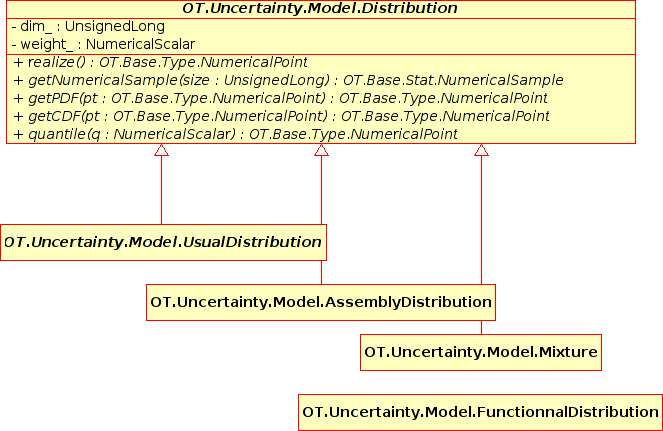
\includegraphics[scale=0.5]{Figures/design/Distribution.png}
    \caption{Distribution, UsualDistribution, AssemblyDistribution, Mixture, and FunctionalDistribution classes.}\label{fig:distribution2}
  \end{center}
\end{figure}

The distribution is a multi-dimensional object within the \OT\ platform, even though the user has direct access only to given dimensions. As it turns out, some distributions may not exist for all possible dimensions of the vectorial space that the user is interested in. This results in an exception being raised for any unimplemented case.

The dimension of a distribution can be accessed with the \emph{dim()} method. Once the distribution is created, it cannot be modified.

A distribution can produce a realization value and return a NumericalPoint with the pure virtual \emph{realize()} method. It can also directly produce a numerical sample of a given size with the pure virtual \emph{getNumericalSample()} method.

The distribution's probability density function and cumulative distribution function can respectively be retrieved with the \emph{getPDF()} and \emph{getCDF()} methods.

The \emph{quantile()} method returns the quantile of a distribution. It has to be noted that this method is only implemented (and only makes sense) for 1-dimensional distributions.

The \emph{weight} parameter is described in the Mixture section (later on in this section).

\paragraph{UsualDistribution}

The UsualDistribution class derives from the abstract Distribution class and defines an interface for all usual distributions supported by the \OT\ platform. Usual distribution means any distribution for which either the analytical form or an evaluation method is known, that can be defined by the user without any information other than the distribution's parameters.

The UsualDistribution class declares a pure virtual method \emph{getKernel()} which returns a Kernel object matching the distribution's kernel. If a class deriving from UsualDistribution has no kernel, an exception is raised.

All distributions deriving from the UsualDistribution class are declared in an independent package, namely OT::Uncertainty::Distribution.

\begin{figure}[htb]
  \begin{center}
    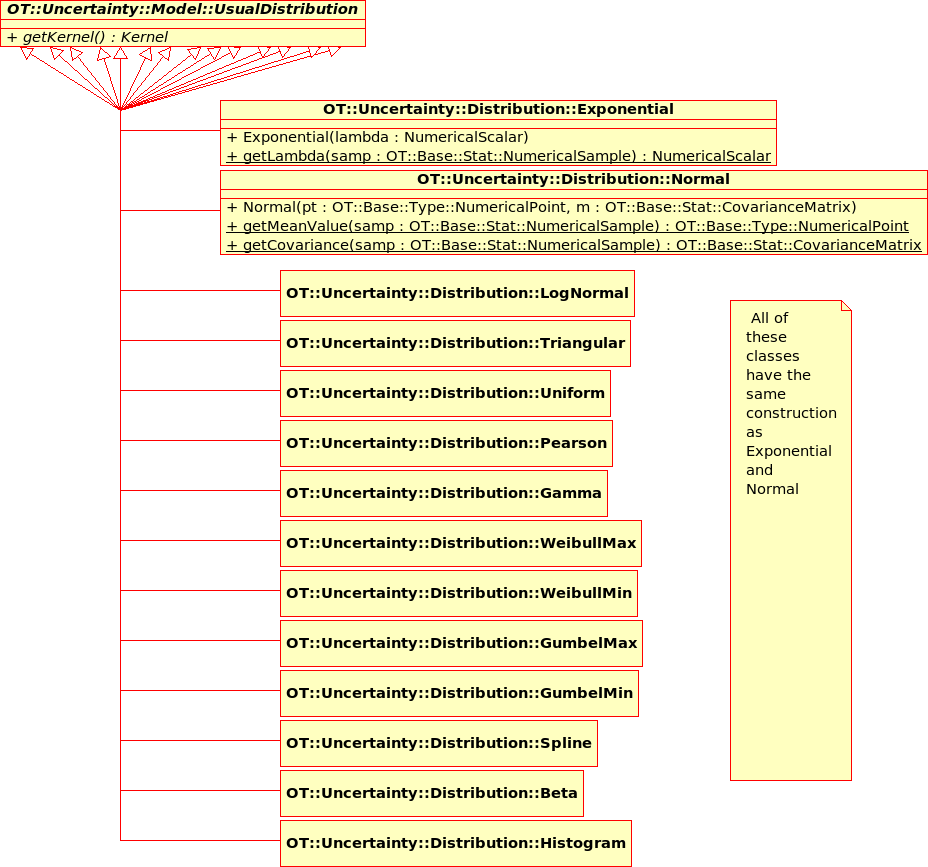
\includegraphics[scale=0.4]{Figures/design/UsualDistribution.png}
    \caption{UsualDistribution and related classes.}\label{fig:usualdist}
  \end{center}
\end{figure}

\paragraph{AssemblyDistribution}

The AssemblyDistribution class, described in Figure \ref{fig:assdist}, derives from the abstract Distribution class and implements the distribution assembly mechanism. To achieve this, it relies on a distribution collection and on a copula which defines the correlation between the collection's distributions. The distribution order in the collection is relevant: it determines the order of the assembly distribution components. The copula's dimension must match the number of components in the distribution collection, which will also the dimension of the final AssemblyDistribution object.

\begin{figure}[htb]
  \begin{center}
    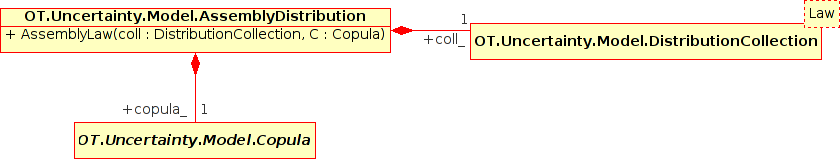
\includegraphics[scale=0.5]{Figures/design/AssemblyDistribution.png}
    \caption{AssemblyDistribution, DistributionCollection and Copula classes.}\label{fig:assdist}
  \end{center}
\end{figure}

\paragraph{Mixture}

The Mixture class derives from the abstract class Distribution and implements the mechanism of mixture distribution (i.e. linear combination of distributions). The analysis showed that it was necessary to draw upon the concept of weighted distribution in order to represent the product of a distribution by the distribution's weight (a numerical scalar) within the linear combination. So as to not introduce another specific class to support the distribution / numerical scalar pair, and since this concept is only used in the platform in this very context, it is not a problem to have the Distribution class directly support this weight (attribute weight).

\begin{figure}[htb]
  \begin{center}
    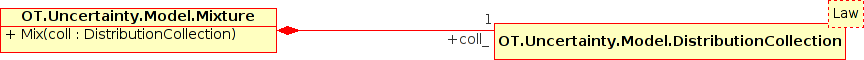
\includegraphics[scale=0.5]{Figures/design/Mixture.png}
    \caption{Mixture and DistributionCollection classes.}\label{fig:mixture}
  \end{center}
\end{figure}

Thus the Mixture class allows to create a linear combination of any distributions, whose weight must be set with the Distribution's \emph{setWeight()} method. The \emph{getWeight()} allows to retrieve this value.

\paragraph{FunctionalDistribution}

The FunctionalDistribution class derives from the abstract Distribution class and implements the transformation mechanism of a distribution through a numerical function. The antecedent distribution belongs to a random vector passed as an argument to the functional distribution when it is created. This class encompasses all of the operations the CompositeRandomVector must support.

\begin{figure}[htb]
  \begin{center}
    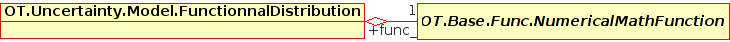
\includegraphics[scale=0.5]{Figures/design/FunctionalDistribution.png}
    \caption{FunctionalDistribution and NumericalMathFunction classes.}\label{fig:funcdist}
  \end{center}
\end{figure}

\paragraph{DistributionCollection}

The distribution collection is implemented by the DistributionCollection class deriving from the Collection class and defining an ordered set of Distribution objects.

\paragraph{DistributionFactory}

The usual distributions (UsualDistribution) can be either directly instantiated by the user, or instantiate through a factory mechanism. The DistributionFactory class implements the latter mechanism according to the Factory pattern described in section \ref{factory}, which shows two parallel class hierarchies. The abstract DistributionFactory class mirrors the UsualDistribution class, and the derived classes of each of these classes are symmetric.

DistributionFactory is an abstract class and, as such, requires to be derived into specific classes for each distribution family. This way, the concept of distribution factory covers the concept of distribution family. Anywhere where the distribution family appears in the analysis model, the distribution factory can be used as an implementation.

The pure virtual method \emph{getDistribution()} generates a usual distribution belonging to the factory's family; to achieve this, it uses either a numerical sample passed as an argument, or a numerical point and a covariance matrix. However, there are different algorithms working out the parameters of the distribution object to be created. These algorithms are determined by the distribution factory policy template parameter (DistributionFactoryPolicy) which is used to instantiate the distribution factory.

The \emph{getKernel()} method allows to retrieve the Kernel object associated with the factory's distribution family.

\begin{figure}[htb]
  \begin{center}
    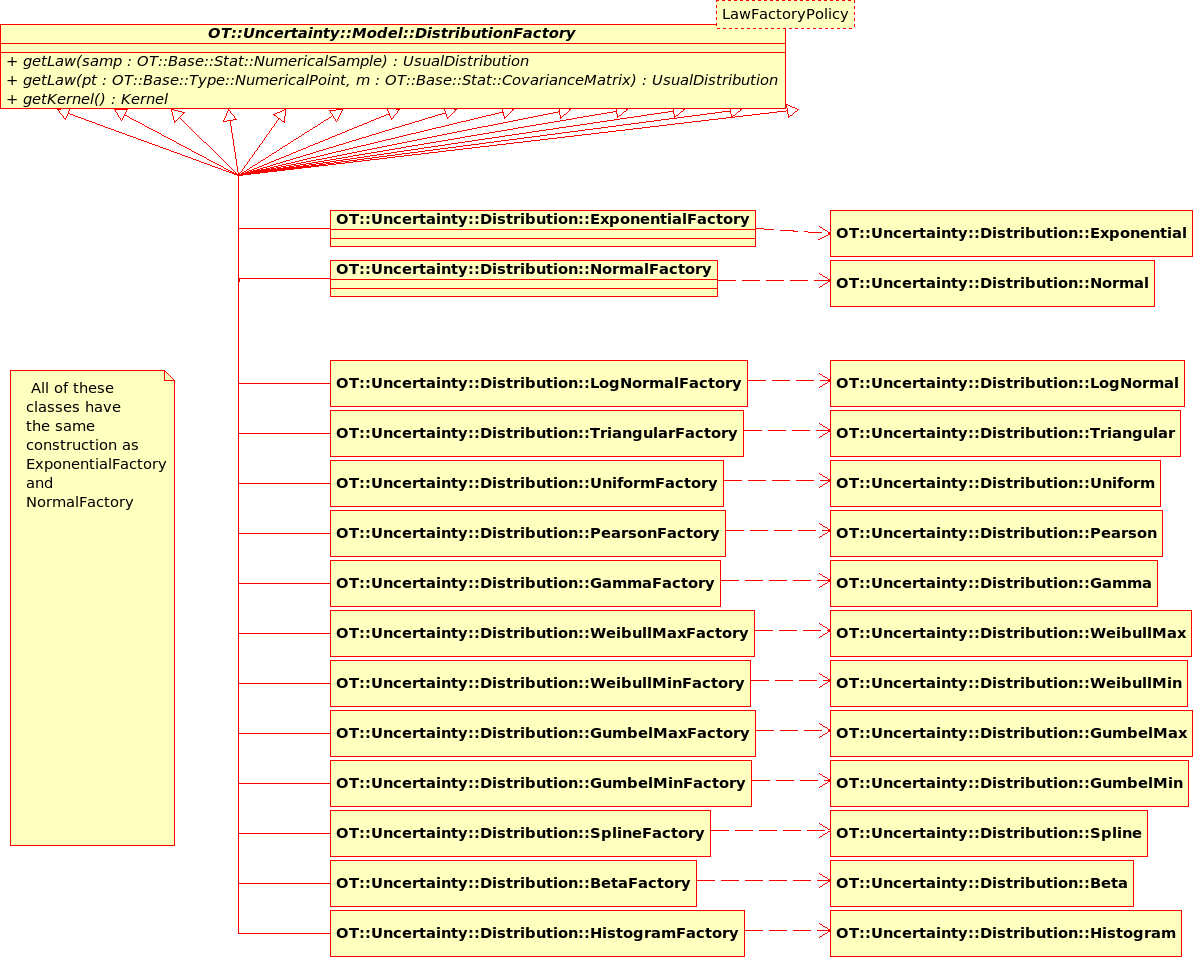
\includegraphics[scale=0.4]{Figures/design/DistributionFactory.png}
    \caption{DistributionFactory and related classes.}\label{fig:distfact}
  \end{center}
\end{figure}

\paragraph{DistributionFactoryPolicy}

As described in Figure \ref{fig:distfactpol} and in the previous section, the DistributionFactoryPolicy class defines an interface for the distribution factory policies.

The DistributionFactoryPolicy is derived into MaximumLikelihood and MomentMethod.

\begin{figure}[htb]
  \begin{center}
    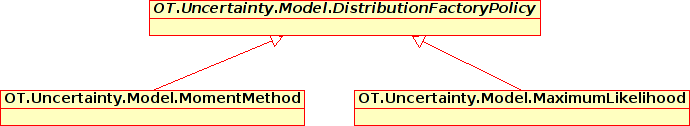
\includegraphics[scale=0.5]{Figures/design/DistributionFactoryPolicy.png}
    \caption{DistributionFactoryPolicy, MomentMethod, and MaximumLikelihood classes.}\label{fig:distfactpol}
  \end{center}
\end{figure}

\paragraph{Kernel}

The Kernel interface gives access to the kernel defined for each usual distribution. Each usual distribution is supposed to return a Kernel object.

This interface defines the legal operations on Kernel objects, which are an \emph{L2Norm()} method which returns the L2 norm of the kernel, and a \emph{covariance()} method which returns the covariance matrix of the said kernel.

This Kernel interface is implemented into as many derived classes as there are usual distributions supported by the platform (see Figure \ref{fig:kernel}). These derived classes all belong to the OT::Uncertainty::Distribution package.

\begin{figure}[htb]
  \begin{center}
    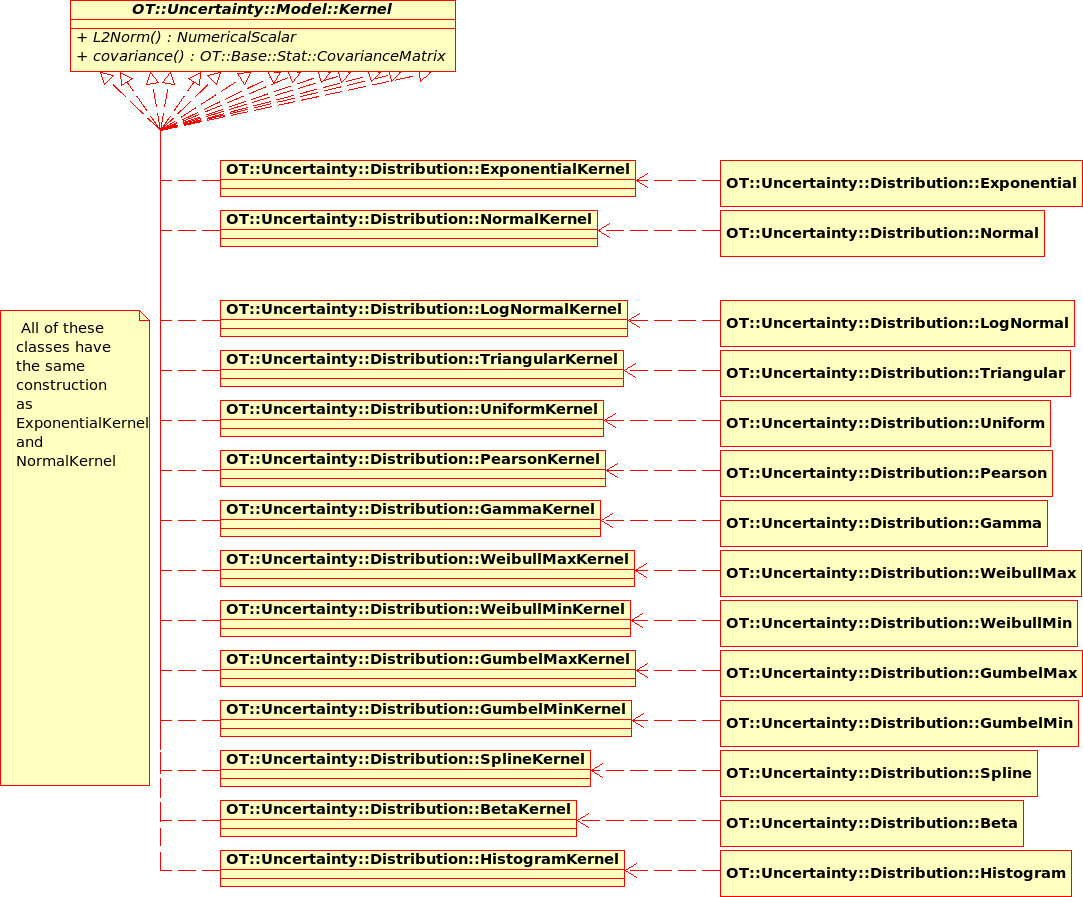
\includegraphics[scale=0.4]{Figures/design/Kernel.png}
    \caption{Kernel and related classes.}\label{fig:kernel}
  \end{center}
\end{figure}

\paragraph{GenericRandomVector}

The GenericRandomVector, described in Figure \ref{fig:randomvector}, defines an interface for all of the tool's random vectors. Though central from the user's point of view and for the mathematical modeling of their study, the concept of random vector is secondary compared to the concept of distribution within the platform. The random vector is rather a concept related to distribution instantiation than an entity in its own right.

However, it differs from the distribution, since it allows to chain random vectors so as to model the dependency that may exist between them. Specifically, a random vector can be built from one or several other random vectors, which defines a dependency tree. This tree itself is modeled with the Composite pattern (see section \ref{composite}).

The GenericRandomVector abstract class defines an interface which must be implemented by the derived classes RandomVector, ConstantRandomVector, CompositeRandomVector, etc.

The random vector implements the methods defined for the distribution. If needed, the execution of these methods can be delegated to an embedded object which offers the user the same interface as the distribution.

A Description may be added to the random vector; it informs the user of the nature of its components.

The \emph{accept()} method allows to launch a RandomVectorVisitor visitor object on a RandomVector object or a derived object. The Visitor pattern is described in section \ref{visitor}.

\begin{figure}[htb]
  \begin{center}
    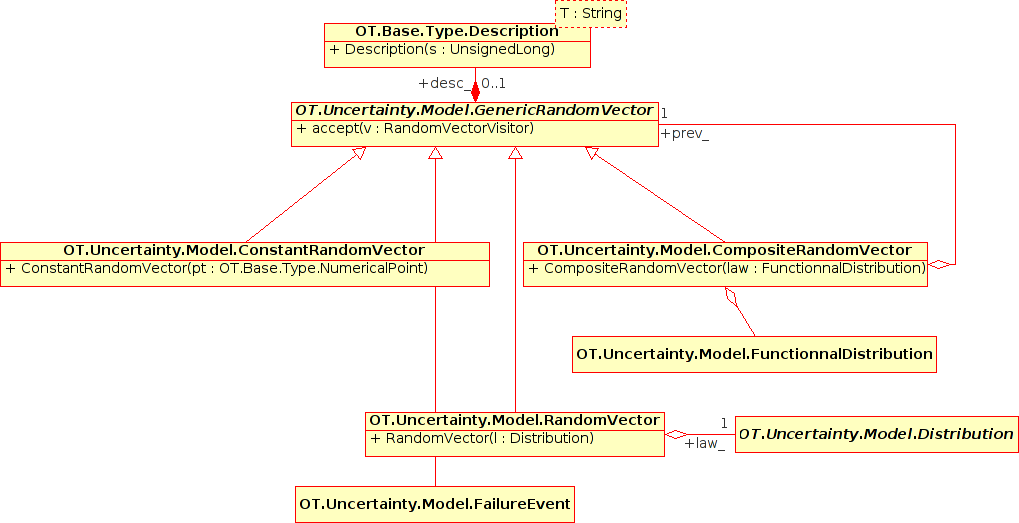
\includegraphics[scale=0.4]{Figures/design/RandomVector.png}
    \caption{GenericRandomVector and related classes.}\label{fig:randomvector}
  \end{center}
\end{figure}

\paragraph{RandomVector}

The RandomVector class, which derives from GenericRandomVector, implements a random vector that can be manipulated by the user. This random vector is defined by a joint distribution.

A random vector is by default built from a distribution (Distribution) which describes its behavior.

\paragraph{ConstantRandomVector}

The ConstantRandomVector, which derives from GenericRandomVector, implements a constant random vector, that is, a vector whose values are all associated with the same numerical point (NumericalPoint).

It is naturally built from a NumericalPoint.

\paragraph{CompositeRandomVector}

The CompositeRandomVector class, which derives from GenericRandomVector, implements a random vector defined on the basis of another random vector and a numerical function. This definition mechanism for random vectors allows the user to model the dependency between the vectors in their study while postponing the computation (the propagation) to a later stage.

The CompositeRandomVector is built on the basis of a GenericRandomVector and a NumericalMathFunction.

It implements a \emph{getNumericalMathFunction()} method which returns the numerical function associated to the CompositeRandomVector. This function cannot be modified once the object is created.

It also provides a \emph{getAntecedent()} method which returns the antecedent random vector on which the composite vector is based. As for the function, the antecedent cannot be modified once the object is created.

\paragraph{Copula}

The Copula class described in Figure \ref{fig:copula} defines a generic interface for all of the copulas that can be implemented in the \OT\ platform. The Copula class is an abstract class.

\begin{figure}[htb]
  \begin{center}
    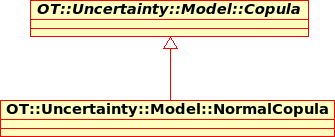
\includegraphics[scale=0.5]{Figures/design/Copula.png}
    \caption{Copula and NormalCopula classes.}\label{fig:copula}
  \end{center}
\end{figure}

\paragraph{NormalCopula}

The NormalCopula class, which derives from Copula, implements a Gaussian copula.

\paragraph{FailureEvent}

The FailureEvent class, described in figures \ref{fig:randomvector} and \ref{fig:failureevent}, is a specialization of GenericRandomVector. It implements the mechanisms related to a failure event.

The FailureEvent class introduces a second Composite pattern within GenericRandomVector's class hierarchy, similar to the one used for CompositeRandomVector.

A FailureEvent object is created from a random vector (GenericRandomVector), a comparison operator (ComparisonOperator), and a threshold (which is a numerical scalar). Because the failure event is itself a random vector whose dimension is 1, the antecedent random vector must have the same dimension. If it is not the case, an exception is raised during the object's creation.

The antecedent of the FailureEvent object can be accessed through the \emph{getAntecedent()} method.

The comparison operator can be accessed through the \emph{getOperator()} method.

The threshold value can be accessed with the \emph{getThreshold()} method.

None of the values or objects used for the construction of the FailureEvent object can be modified once the object is created.

\begin{figure}[htb]
  \begin{center}
    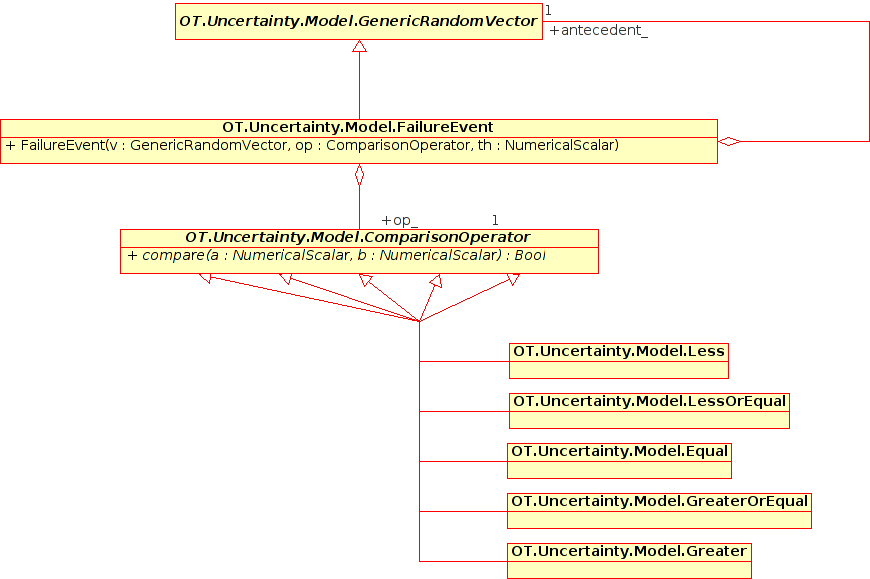
\includegraphics[scale=0.5]{Figures/design/FailureEvent.png}
    \caption{FailureEvent class.}\label{fig:failureevent}
  \end{center}
\end{figure}

\paragraph{ComparisonOperator}

The FailureEvent objects rely on a comparison mechanism between the vector's value and a numerical scalar designated as the threshold. So as to be able to pass any type of comparison operator do the failure event, the \OT\ platform provides an abstract class, ComparisonOperator, which defines the interface that any comparison operator must support.

Thus the class defines a pure virtual method \emph{compare()} which compares two numerical scalars and returns a Bool whose value depends on the outcome of the comparison.

The ComparisonOperator class is derived into Less, LessOrEqual, Equal, GreaterOrEqual, and Greater.

\paragraph{Less}

The Less class, deriving from ComparisonOperator, implements the "less than" comparison.

\paragraph{LessOrEqual}

The LessOrEqual class, deriving from ComparisonOperator, implements the "less than or equal" comparison.

\paragraph{Equal}

The Equal class, deriving from ComparisonOperator, implements the "equal to" comparison.

\paragraph{GreaterOrEqual}

The GreaterOrEqual class, deriving from ComparisonOperator, implements the "greater than or equal to" comparison.

\paragraph{Greater}

The Greater class, deriving from ComparisonOperator, implements the "greater than" comparison.

\paragraph{MaximumLikelihood}

The MaximumLikelihood class, deriving from DistributionFactoryPolicy, implements an algorithm that computes the parameters of a usual distribution (UsualDistribution) using the method of maximum likelihood. This class is used to provide parameters for the DistributionFactoryPolicy instances.

\paragraph{MomentMethod}

The MomentMethod class, deriving from DistributionFactoryPolicy, implements an algorithm that computes the parameters of a usual distribution (UsualDistribution) using the method of moments. This class is used to provide parameters for the DistributionFactoryPolicy instances.

\paragraph{RandomVectorIterator}

The RandomVectorIterator naturally derives from Iterator. It allows to travers the dependency tree of a random vector by visiting each child of each vector. However, the dependency tree of a vector is an acyclic oriented graph by construction, thus one child may be visited several times by the iterator in case of multiple dependencies.

\begin{figure}[htb]
  \begin{center}
    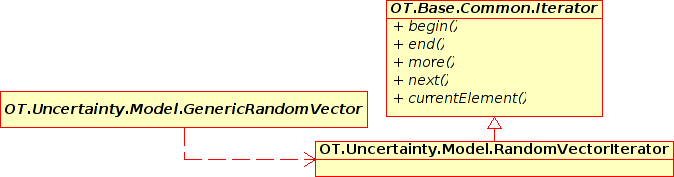
\includegraphics[scale=0.5]{Figures/design/RandomVectorIterator.png}
    \caption{Iterator, RandomVectorIterator and GenericRandomVector classes.}\label{fig:rviterator}
  \end{center}
\end{figure}

\paragraph{OptimalWalkIterator}

The OptimalWalkIterator class derives from Iterator. Objects of this type are produced by an OptimalWalkVisitor which determines the optimal path to traverse the dependency graph of a random vector. During the traversal it controls, the object does not guarantee access to all of the graph's elements. Actually, it is quite the contrary: the goal of such an object is to reduce the tree so as to optimize a criterion determined by the OptimalWalkVisitor object.

\paragraph{RandomVectorVisitor}

The RandomVectorVisitor class defines an interface for all visitors of the class hierarchy stemming from GenericRandomVector. It implements the Visitor pattern described in section \ref{visitor}.

\begin{figure}[htb]
  \begin{center}
    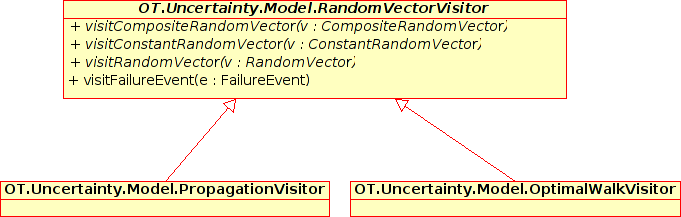
\includegraphics[scale=0.5]{Figures/design/RandomVectorVisitor.png}
    \caption{RandomVectorVisitor, PropagationVisitor and OptimalWalkVisitor classes.}\label{fig:rvvisitor}
  \end{center}
\end{figure}

The RandomVectorVisitor class is an abstract class. All of its methods are pure virtual methods and they must be re-defined in the derived classes.

The methods \emph{visitCompositeRandomVector()}, \emph{visitConstantRandomVector()}, \emph{visitRandomVector()}, \emph{visitFailureEvent()}, etc. are implemented according to the processing that must be performed for each type of random vector.

\paragraph{OptimalWalkVisitor}

The OptimalWalkVisitor class, which derives from RandomVectorVisitor, performs a complete traversal of the dependency tree of a random vector; this allows to determine the order in which the tree's vectors must be traversed so as to optimize a given criterion (internal to the visitor, such as limiting the memory usage, not re-evaluating a vector, etc.).

The OptimalWalkVisitor class generates an OptimalWalkIterator specific to the new traversal path.

This path can be used to ensure the propagation of uncertainties within the dependency tree, for example with the help of a PropagationVisitor.

\paragraph{PropagationVisitor}

The PropagationVisitor class, which derives from RandomVectorVisitor, allows to propagate uncertainties within the dependency graph of a random vector while relying on the optimal traversal determined by an OptimalWalkVisitor.

\subsubsection{Distributions}

These elements belong to the Uncertainty/Distribution/ sub-folder of the source tree.

The distributions described in this section are the usual distributions known to the platform. Table \ref{distributiontable} describes the mapping between the distribution's name and the class prefix used within the \OT\ platform.

\begin{center}
  \begin{table}[h]
    \caption{\label{distributiontable}Mapping between distributions and classes}
    \begin{center}
      \begin{tabular}{|l|l|}
        \hline
        \textbf{Usual name of the distribution} & \textbf{Class prefix (XDistribution)} \\
        \hline \hline
        B�ta & Beta \\
        Exponential & Exponential \\
        Gamma & Gamma \\
        Gumbel & Gumbel \\
        Histogram & Histogram \\
        Log normal & LogNormal \\
        Log uniform & LogUniform \\
        Normal & Normal \\
        Pearson & Pearson \\
        Spline & Spline \\
        Triangular & Triangular \\
        Uniform & Uniform \\
        Weibull& Weibull \\
        \hline
      \end{tabular}
    \end{center}
  \end{table}
\end{center}

\paragraph{XDistribution}

Each XDistribution implements a usual distribution as defined in the methodological reference of \OT\ (see \cite{OTmeth}). These distributions are objects that can be directly manipulated by the user. They can be created using a set of parameters, each parameter set specifically depending on the XDistribution.

Each XDistribution also provides a \emph{getKernel()} method which returns a Kernel object specific to XDistribution. This object cannot be modified: it is statically defined in the platform.

\paragraph{XDistributionFactory}

According to the Factory design pattern (see section \ref{fig:class}), each XDistribution possesses a factory called XDistributionFactory, which allows to instantiate any distribution from the XDistribution class.

Each XDistributionFactory class defines a set of \emph{getDistribution()} methods (which makes use of the exact same parameters defined for each XDistribution) as well as a \emph{getKernel()} method which returns the Kernel object specific to XDistribution.

\paragraph{XDistributionKernel}

Each XDistribution should define a Kernel object specific to the distribution. Given the unicity and the specificity of this object on the one hand, and its state-less characteristic on the other, it is statically declared in the \OT\ platform. The object XDistributionKernel defines the methods declared in the Kernel interface.

\subsubsection{Simulation algorithms}

This package encompasses all classes implementing the uncertainty propagation algorithms offered by the \OT\ platform. These classes rely on a model of the problem created with the help of classes from the Model and Distribution packages. These elements belong to the namespace OT::Uncertainty::Algorithm.

\paragraph{UncertaintyAlgorithm}

Figure \ref{fig:uncertainty} shows the hierarchy of simulation algorithm classes, at the head of which is the abstract class UncertaintyAlgorithm. This class defines a common interface to all of the platform's algorithms.

\begin{figure}[htb]
  \begin{center}
    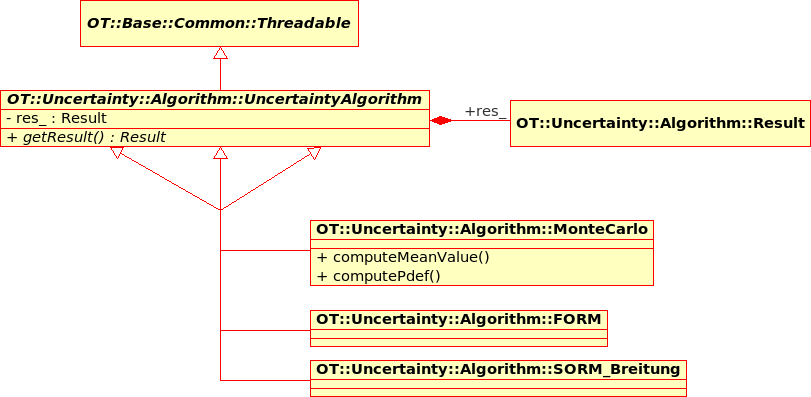
\includegraphics[scale=0.5]{Figures/design/UncertaintyAlgorithm.png}
    \caption{UncertaintyAlgorithm, Result, Threadable and related classes.}\label{fig:uncertainty}
  \end{center}
\end{figure}

The UncertaintyAlgorithm class derives from the Threadable class. Threadable defines a \emph{run()} method within which the given algorithm must be implemented. Since a Thread object can handle it, such an algorithm can be used within the platform parallelly to other operations the user may want to carry out. However, this requires to handle the multi-threading aspects within the UncertaintyAlgorithm class in an appropriate manner, particularly as far as concurrent access to shared data (e.g. internal state) is concerned; if it is not dealt with appropriately, the risk is to produce inconsistent results, or even to crash the platform. Therefore (and unless explicitely mentioned), any of this class's methods must be multithread-safe.

When the computation taking place within the \emph{run()} method is completed, the result can be accessed in a Result object returned by the pure virtual method \emph{getResult()}.

\paragraph{Result}

The Result class defines the broad set of results that can be produced by a simulation algorithm. The default behavior is to create an empty Result object. It must be completed by adding data as the study progresses. Since access to this object can be performed within a multi-threaded procedure, the object needs to be protected from concurrent access. It possesses an internal lock to which its accessor must refer.

Details about the data that can be stored in a Result object will be given in a future version of this document.

\paragraph{MonteCarlo}

The Monte-Carlo class derives from UncertaintyAlgorithm and implements a Monte-Carlo algorithm to propagate uncertainties. It is described in Figure \ref{fig:montecarlo}.

\begin{figure}[htb]
  \begin{center}
    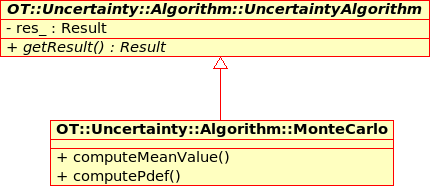
\includegraphics[scale=0.5]{Figures/design/MonteCarlo.png}
    \caption{UncertaintyAlgorithm and MonteCarlo classes.}\label{fig:montecarlo}
  \end{center}
\end{figure}

It defines several methods indicating which data should appear in the final Result object.

The \emph{computeMeanValue()} method triggers the computation of the vector's mean value.

The \emph{computePdef()} method triggers the computation of the event's probability of failure (the event being a vector).

\paragraph{FORM}
The FORM class derives from UncertaintyAlgorithm and implements a FORM algorithm to propagate uncertainties. It is described in Figure \ref{fig:form}.

\begin{figure}[htb]
  \begin{center}
    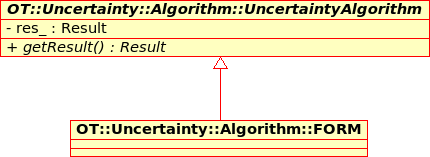
\includegraphics[scale=0.5]{Figures/design/FORM.png}
    \caption{UncertaintyAlgorithm and FORM classes.}\label{fig:form}
  \end{center}
\end{figure}

It defines several methods indicating which data should appear in the final Result object.

\paragraph{SORM\_Breitung}

The SORM\_Breitung class derives from UncertaintyAlgorithm and implements a SORM algorithm to propagate uncertainties. It is described in Figure \ref{fig:sorm}.

\begin{figure}[htb]
  \begin{center}
    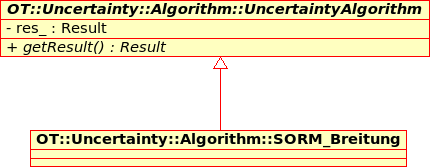
\includegraphics[scale=0.5]{Figures/design/SORM_Breitung.png}
    \caption{UncertaintyAlgorithm and SORM\_Breitung classes.}\label{fig:sorm}
  \end{center}
\end{figure}

It defines several methods indicating which data should appear in the final Result object.
